\chapter{The Persistent Distributed Agent-Based Genetic Algorithm}
  The Persistent Distributed Agent-Based Genetic Algorithm (PDABGA) 
    is an island-type distributed genetic algorithm (GA). 
  The general goal for the new algorithm are to optimize extremely
    complex problems utilizing a distributed network of computing hosts
    over an indefinite period of time.
  These goals are accomplished by utilizing mobile-agent technology in the 
    design of the algorithm.

  The population of the of the GA is composed of autonomous mobile agents.
  Each agent in the agent population is responsible for its own fitness
    calculation, mate selection, and reproduction.
  PDABGA is
    comprised of a handful of individual components, including a Mobile-C
    agency, various Mobile-C agents, a simulation framework, and a
    newscast network binding the distributed agencies together, as summarized
    in Figure \ref{fig:pdabga_architecture}.
  The following sections will disseminate each of the components in detail.

  % FIGURE --------------------------------------------------
  \begin{figure}[!ht]
  \begin{center}
     \includegraphics[width=5in]{figures/application_architecture}
  \end{center}
  \caption{\label{fig:pdabga_architecture}Application architecture of a PDABGA agency.}
  \end{figure}
  % END FIG -------------------------------------------------


  \section{Mobile-C: A C/C++ Mobile Agent Framework}
    Mobile-C was first conceived and prototyped as a standalone application which
      processed agents written in C embedded in XML \cite{chen2005}. 
    During the course of this research, it has evolved to become an embeddable,
      fast, and stable agent platform. 
    Mobile-C has already been used in several robotic systems, such as robotic
      workcells \cite{Nestinge2010b}. 
    In the robotic workcells, the agents take advantage of agent
      synchronization methods provided by Mobile-C to perform a coordinated task.
    Mobile-C has also been used on mobile robots performing distributed vision
      sensor fusion \cite{Nestinge2010}. 
    By utilizing mobile agents, image processing is done in situ on the robots,
      thereby saving network bandwidth and energy.

  \section{Agency Design}
    \subsection{Synopsis}
      The agency is a complex engine, housing multiple mobile and stationary
        agents that interact with each other. 
      The following is a brief synopsis of the typical workflow of a PDABGA
        agency. 
      
      \begin{enumerate}
        \item The agency initializes. This involves starting the Master agent,
          Cull agent, Newscast agent, and a number of initial Worker agents.
        \item The initial Worker agents are started with randomized genes and 
          unknown fitnesses. 
        \item Any Worker agent checks to see if it has a saved fitness upon
          startup. If there is no fitness saved, it requests to run a gait
          simulation to find its fitness. If there are too many simulation
          processes running, the agent waits in line for other simulation
          processes to end.
        \item Once a Worker agent finds its fitness, it asks the Master agent
          for a list of its peers. 
        \item The worker picks potential mates from the list according to
          a selection algorithm and sends requests to mate. 
        \item If a mating request is successfull, the worker that initiated 
          the request performs the crossover algorithm on the parent chromosomes
          and sends the result to the Master agent.
        \item The Master agent schedules creation of a new agent with the new
          chromosomes.
        \item Occasionally, the Cull agent will check the total number of
          agents on the system. If the number of agents exceeds a predetermined
          maximum, agents with inferior fitness are terminated by the Cull agent.
        \item Occasionally, the Newscast agent will contact other Newscast agents
          running on other agencies to maintain a well-connect newscast network
          among agencies.
        \item Occasionally, worker agents will communicate with the Newscast agent
          and migrate to other agencies.
      \end{enumerate}
      
    \subsection{Initialization}
      The Agency performs a variety of steps upon startup.
      First and foremost, the agency initializes a number of agents which
        perform the bulk of the work during execution of the genetic algorithm.
      These include the Master agent, Cull agent, Newscast agent, and Worker
        agents.

    \subsection{Simulation Manager}
      The cost function is implemented as a separate application and is executed
        as a separate process. 
      By executing the cost function as a separate process, crashes which may occur
        during the simulation will not affect the stability of the whole agency. 
      Furthermore, by executing the cost function as a separate process, the agency
        can take full advantage of multi-core and/or multi-cpu computer systems by
        running a separate simulation process on each core. 
      The Simulation Manager limits the maximum number of running simulations to the
        number of CPU cores on the system.


  \section{Mobile Agent Design}
    \subsection{The Worker Agents}
    Each GA Agent within the PDABGA is analagous to a living entity in the real world.
    The agents carry genetic material, can travel to new locations, look for
      mates, have children, and susceptible to death depending on their fitness.
    \subsubsection{Initialization}
      % FIGURE --------------------------------------------------
      \begin{figure}[!ht]
      \begin{center}
         \includegraphics[width=3in]{figures/worker_agent_init}
      \end{center}
      \caption{\label{fig:worker_agent_init}Worker agent initialization.}
      \end{figure}
      % END FIG -------------------------------------------------

      Upon startup, the agents perform an initialization process, as shown
      in Figure \ref{fig:worker_agent_init}.
      First, the agent checks to see if it has saved chromosomes. 
      An agent that had just migrated to another agency will have saved
        chromosomes from its life on the previous agency. 

    The agents are implemented as a state machine capable of carrying multiple
      conversations simultaneously with other agents and agencies. 
    The state machine is summarized in Figure \ref{fig:gaAgentStateMachine}.
    Note that the state machine is implemented on a per-conversation basis, such that
      multiple conversations can be maintained by a single agent simultaneously. 

      % FIGURE --------------------------------------------------
      \begin{figure}[!ht]
      \begin{center}
         \includegraphics[width=5in]{figures/convo_state_diagram}
      \end{center}
      \caption{\label{fig:gaAgentStateMachine}Worker agent conversation state machine.}
      \end{figure}
      % END FIG -------------------------------------------------
    

    \subsection{The Master Coordinator Agent}

    \subsection{The Cull Agent}

    \subsection{The Newscast Agent}


